\section{Verhalten eines Magneten beim Fall durch ein Aluminiumrohr mit und ohne Schlitz.}

Dieses Experiment untersucht das gleiche verhalten das auch schon in \cref{kap:Kamm_Platte} zu beobachten war.
Hier wurde ein Magnet erst durch ein Rohr ohne Unterbrechungen in der Mantelfläche fallen gelassen und danach durch ein Rohr das an der Seite einen Schlitz hatte sodass die Oberfläche vollständig unterbrochen war (vgl. \cref{fig:Rohr}).
Beobachtet wurde bei der Durchführung das der Magnet durch das nicht ganz geschlossene Rohr zwar Langsamer fällt als wenn man ihn einfach so fallen gelassen hätte. Jedoch deutlich schneller als durch das Rohr mit dem nicht durchbrochenem Mantel. Dies ist eben genau auf diese Unterbrechung zurückzuführen, denn diese verhindert das schon in\cref{kap:Kamm_Platte} angesprochene induzieren von Wirbelströmen auf die Oberfläche des Rohrs. Da dies verhindert wurde ist der auftretende Paramagnetische Effekt ungleich kleiner als bei der Vollständig geschlossenen Röhre wo dies möglich ist. 
\begin{figure}[h]
	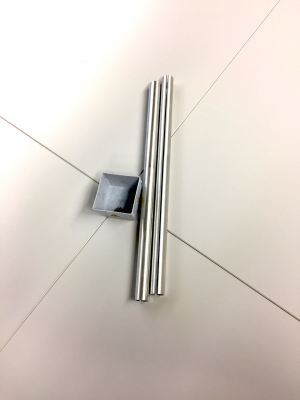
\includegraphics[width=0.5\textwidth]{res/Rohr.png}
	\caption{In dieser Abbildung sind die in diesem Experiment verwendeten Aluminiumrohre zu sehen\protect\footnotemark.}
	\label{fig:Rohr}
\end{figure}
\footnotetext{Entnommen am 20.11.17  aus dem Learnweb Kurs "Experimentelle Übungen I 17-18"}